	\documentclass[aspectratio=43]{beamer}
\usepackage[english]{babel}
\usepackage{amsthm}
\usepackage{amsfonts}
\usepackage{amsmath}
\usepackage{amssymb}
\usepackage{mathtools}
\usepackage{bbm}
\usepackage{pgfplots}
\usepackage{tikz}
%\usepackage{physics}
\usepackage{calligra}
\usepackage{csquotes}
%\usepackage{tensor}
\usepackage[thicklines]{cancel}
\usepackage{tcolorbox}
%\usepackage{pstricks}
\usepackage[backend=biber, bibstyle=nature, sorting=nty, citestyle=numeric-comp]{biblatex} %Custom bibliography
    \addbibresource{bib.bib} %Load references
\usepackage{chronology}
\usepackage{msc}

\DeclareMathAlphabet{\mathcalligra}{T1}{calligra}{m}{n}
\DeclareFontShape{T1}{calligra}{m}{n}{<->s*[2.2]callig15}{}
\newcommand{\scriptr}{\mathcalligra{r}\,}
\newcommand{\boldscriptr}{\pmb{\mathcalligra{r}}\,}
\def\rc{\scriptr}
\def\brc{\boldscriptr}
\def\hrc{\hat\brc}
\newcommand{\ie}{\emph{i.e.}} %id est
\newcommand{\eg}{\emph{e.g.}} %exempli gratia
\newcommand{\rtd}[1]{\ensuremath{\left\lfloor #1 \right\rfloor}}
\newcommand{\dirac}[1]{\ensuremath{\delta \left( #1 \right)}}
\newcommand{\diract}[1]{\ensuremath{\delta^3 \left( #1 \right)}}
\newcommand{\e}{\ensuremath{\epsilon_0}}
\newcommand{\m}{\ensuremath{\mu_0}}
\newcommand{\V}{\ensuremath{\mathcal{V}}}
\newcommand{\prnt}[1]{\ensuremath{\left(#1\right)}} %parentheses
\newcommand{\colch}[1]{\ensuremath{\left[#1\right]}} %square brackets
\newcommand{\chave}[1]{\ensuremath{\left\{#1\right\}}}  %curly brackets
\newcommand\eqdef{\stackrel{\mathclap{\normalfont \tiny\mbox{\textrm{def}}}}{=}}
\useoutertheme{infolines}
\useinnertheme{rectangles}
\usefonttheme{professionalfonts}


\definecolor{blue2}{HTML}{045FB4}
\definecolor{green2}{HTML}{46C235}
\definecolor{red2}{HTML}{EE4848}
\definecolor{violet2}{HTML}{A647E5}
\definecolor{orange2}{HTML}{FF7425}
\definecolor{darkred}{HTML}{5C2020}
\definecolor{gray}{HTML}{303030}
\definecolor{yellow}{HTML}{f0be52}
\definecolor{lightdarkgold}{HTML}{EEBC1D}

\renewcommand{\CancelColor}{\color{darkred}}

\makeatletter
\newcommand{\mybox}[1]{%
  \setbox0=\hbox{#1}%
  \setlength{\@tempdima}{\dimexpr\wd0+13pt}%
  \begin{tcolorbox}[colback=gray,colframe=gray,boxrule=0.5pt,arc=4pt,
      left=6pt,right=6pt,top=6pt,bottom=6pt,boxsep=0pt,width=\@tempdima]
    \textcolor{yellow}{#1}
  \end{tcolorbox}
}
\makeatother


\pgfplotsset{my style/.append style={axis x line=middle, axis y line=
middle, xlabel={$x$}, ylabel={$y$}, axis equal }}


\usecolortheme[named=gray]{structure}
\usecolortheme{sidebartab}
\usecolortheme{orchid}
\usecolortheme{whale}
\setbeamercolor{titlelike}{parent=structure, bg=structure, fg=white}
\setbeamercolor{section in toc}{fg= white}
\setbeamercolor{subsection in toc}{fg= white}
%\setbeamercolor*{sidebar}{fg=red2,bg=gray!15!white}

\setbeamercolor{item projected}{bg=yellow, fg = gray}
\setbeamertemplate{enumerate items}[default]
\setbeamertemplate{navigation symbols}{}
\setbeamercolor{local structure}{fg=yellow}

\setbeamercolor{alerted text}{fg=white}
\setbeamercolor{block title}{bg = yellow}
\setbeamercolor{block title alerted}{bg=red2}
\setbeamercolor{block title example}{bg=green2}
\setbeamercolor{background canvas}{bg=gray}
\setbeamercolor{normal text}{bg=gray,fg=white}


\setbeamertemplate{footline}
        {
      \leavevmode%
      \hbox{%
      \begin{beamercolorbox}[wd=.333333\paperwidth,ht=2.25ex,dp=1ex,center]{author in head/foot}%
        \usebeamerfont{author in head/foot}\insertshortauthor~~(\insertshortinstitute)
      \end{beamercolorbox}%
      \begin{beamercolorbox}[wd=.333333\paperwidth,ht=2.25ex,dp=1ex,center]{title in head/foot}%
        \usebeamerfont{title in head/foot}\insertshorttitle
      \end{beamercolorbox}%
      \begin{beamercolorbox}[wd=.333333\paperwidth,ht=2.25ex,dp=1ex,center]{date in head/foot}%
        \usebeamerfont{date in head/foot}\insertshortdate{}%\hspace*{2em}

    %#turning the next line into a comment, erases the frame numbers
        %\insertframenumber{} / \inserttotalframenumber\hspace*{2ex} 

      \end{beamercolorbox}}%
      \vskip0pt%
    }


\setbeamertemplate{blocks}[rectangle]
\setbeamercovered{dynamic}




%\setbeamercolor{author}{fg=yellow}
%\setbeamercolor{title}{fg = yellow}
%\setbeamerfont{title}{size=\Large, series=\bfseries}
%\setbeamerfont{author}{size=\footnotesize}
%\setbeamerfont{date}{size=\small}


\setbeamertemplate{section page}
{
	\begin{centering}
		\begin{beamercolorbox}[sep=27pt,center]{part title}
			\usebeamerfont{section title}\insertsection\par
			\usebeamerfont{subsection title}\insertsubsection\par
		\end{beamercolorbox}
	\end{centering}
}





%\setbeamertemplate{subsection page}
%{
%	\begin{centering}
%		\begin{beamercolorbox}[sep=12pt,center]{part title}
%			\usebeamerfont{subsection title}\insertsubsection\par
%		\end{beamercolorbox}
%	\end{centering}
%}

\newcommand{\hlight}[1]{\colorbox{violet!50}{#1}}
\newcommand{\hlighta}[1]{\colorbox{darkred!50}{#1}}


\definecolor{cyan}{rgb}{.63,.79,.95}

    \setbeamertemplate{background} 
    {
        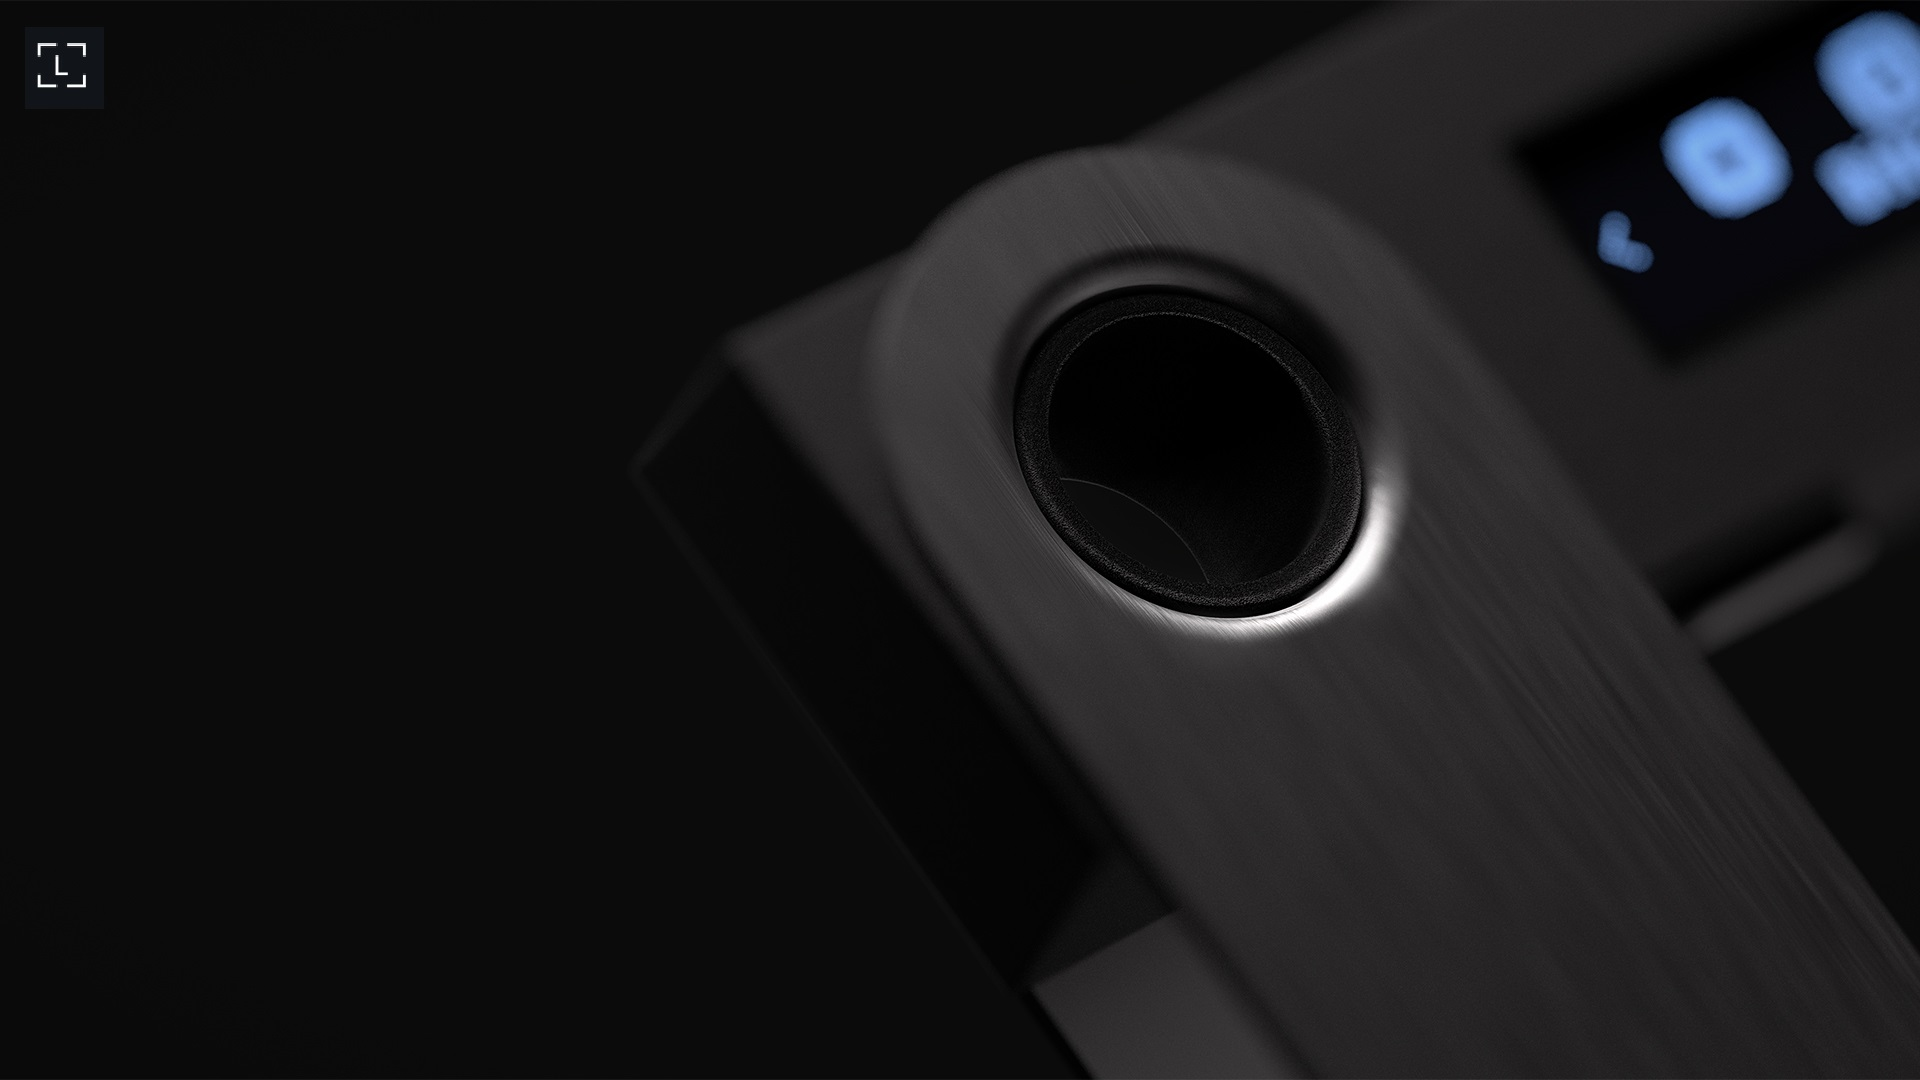
\includegraphics[width=\paperwidth,height=\paperheight]{images/fond1.jpg}
    }
\title{ECDAA for Anonymous Genuine Checks and Signatures} %->->->->-> Check hyperref title <-<-<-<-<-
\subtitle{(Elliptic Curve Anonymous Attestation)}
\author[R. Dubois]{\textcolor{yellow}{Renaud Dubois} }
\institute[LIT]{
    \textcolor{white}{Ledger Innovation Team}%
    \\%
    \textcolor{white}{Saint-Jean-Aux-Bois Crypt2023}%
    \date{\today}
    
    
} %You can change the Institution if you are from somewhere else


%\logo{\includegraphics[width= 0.05\textwidth]{images/logo.png}}

\begin{document}
    
    \frame{\titlepage }
   

%%%%%%%%%%%%         
    \begin{frame}{The Fight for Privacy}
     
     \only<1>{
     \begin{alertblock}{Stakes}
     \begin{itemize}
     \item Threat 1 : value your privacy or you're the product
     
	\begin{center}
	
\includegraphics[width=2cm]{images/dark_barcode.jpg}
	\end{center}
     
     \item Threat 2 : Legislator surveillance
      \begin{center}
	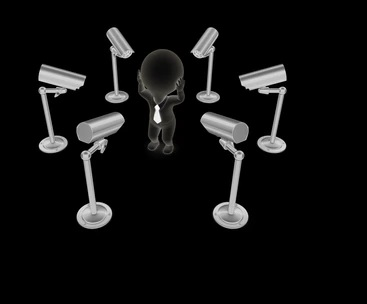
\includegraphics[width=2.5cm]{images/dark_surveillance.jpg}
	\end{center}
     
     \end{itemize}
     \end{alertblock}
     }
     \only<2>{
     \begin{block}{Examples}
     \begin{itemize}
     \item Correlate Ledger Live logs (our DB): links the accounts
     \item identification of the Device public key at genuine check: what about metadata 
     \end{itemize}
     \end{block}
    }    
   
    \end{frame}
     
%%%%%%%%%%%% 

%%%%%%%%%%%%         
    \begin{frame}{Summary}
     
   
        \tableofcontents
   
    \end{frame} 
%%%%%%%%%%%% 
    \section{Anonymous Signatures}

    \begin{frame}{Signatures schemes}
     
     \begin{center}
     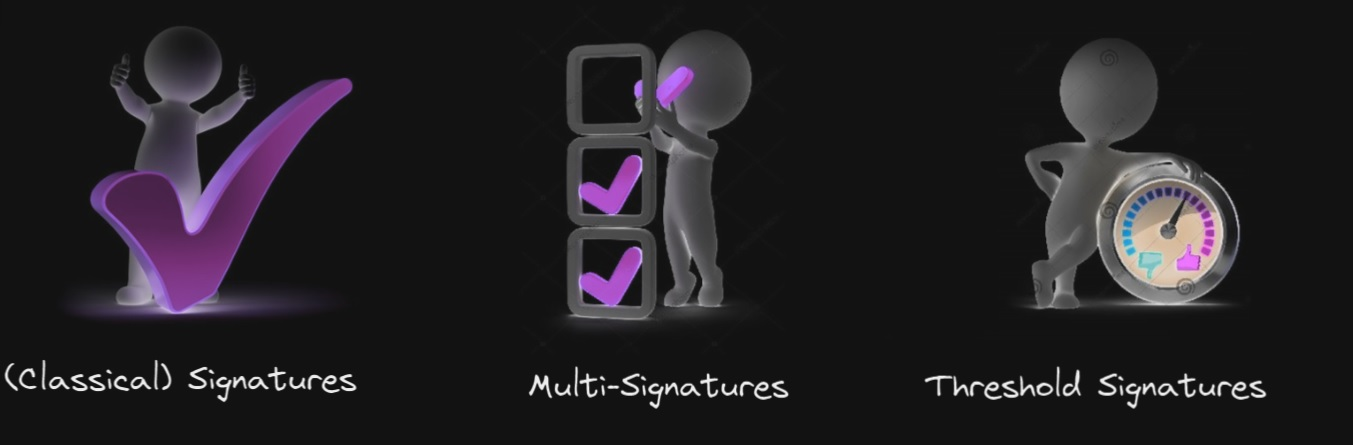
\includegraphics[width=12cm]{images/concepts.jpg}
     
     \begin{tabular}{c c c}
     ~~~~~~~ECDSA \hskip2cm~ & ~~Musig2 \hskip2cm~& FROST \hskip2cm~\\
     \end{tabular}
     \end{center}
     
      {\cyan{\href{https://blog.ledger.com/ring-signature/}{\cyan{Starknet meetup presentation}}}}
 
     
     \end{frame}
%%%%%%%%%%%% 
 \subsection{Properties and Families}
 \begin{frame}{Anonymous Signatures schemes}
 
 \begin{center}
	
\includegraphics[width=1.8cm]{images/anonymous.jpg}
	\end{center}
     
     
   \only<1>{
   \begin{block}{Additional properties}
     \begin{itemize}
     \item  group anonymity : The required anonymity property is that it is impossible for the verifier to identify from which member of the group the signature was issued.
     \item  linkability: enables an entity to identify if two signatures of the same message have been issued by the same user, without knowing the identity of that user.
     
     \end{itemize}
 \end{block}
   }
   \only<2>
   {
   \begin{block}{Schemes}
     \begin{itemize}
     \item  Decentralized :  {\cyan{\href{https://blog.ledger.com/ring-signature/}{Ring Signatures, Linkable Ring Signatures (blog post).}}}
 
     \item Centralized : Anonymous Attestations  
      
     \end{itemize}
     \end{block}
     
     In Decentralized schemes, user select the Ring, in centralized there is an additional entity: the issuer.
   }
   
 \end{frame}  

%%%%%%%%%%%% 
\subsection{ECDAA}
\begin{frame}{Anonymous Credentials}
 
 
 \begin{center}
 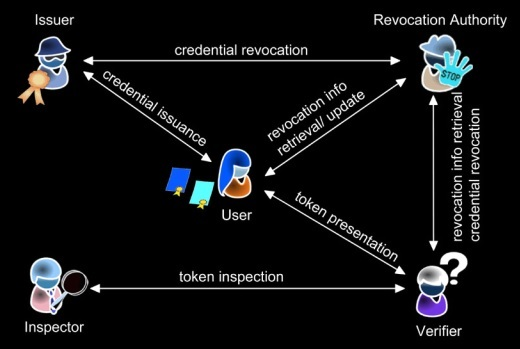
\includegraphics[width=10cm]{images/AnonymousCredentials.jpg}
 \end{center}


 
\end{frame}
%%%%%%%%%%%% 
\begin{frame}{ECDAA}


ECDAA is anonymous, linkable and centralized.


{\cyan \href{https://fidoalliance.org/specs/common-specs/fido-ecdaa-algorithm-v2.1-rd-20210525.pdf}{FIDO 2 draft}}

 \begin{center}
 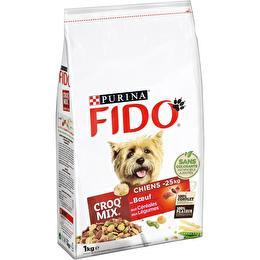
\includegraphics[width=2cm]{images/fido.jpg}
 \end{center}

{\cyan{\href{https://trustedcomputinggroup.org/resource/tpm-library-specification/}{TCG (Trusted Computing Group)}}}
 \begin{center}
 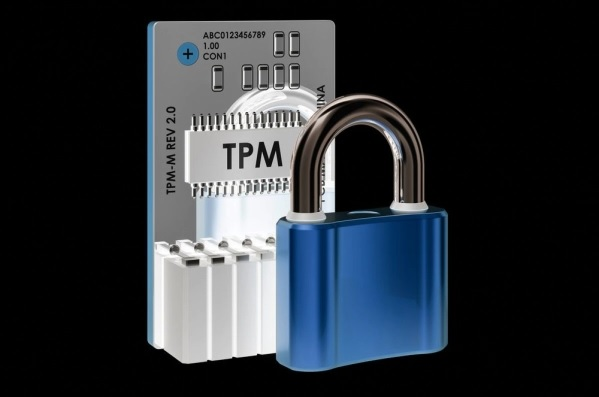
\includegraphics[width=3cm]{images/tpm.jpg}
 \end{center}

It uses advanced cryptographic mechanisms: pairing over elliptic curves.


\end{frame}

\begin{frame}

\tiny{

{\tt{



{\cyan

CREDENTIALS GENERATION

input (sk\_x, sk\_y): issuer secret key

 m, B, Q, c1, s1, n credential received from user 
 
 }
def Issuer\_Gen\_Credentials(sk\_x, sk\_y, m, B, Q, c1, s1, n):
 return A,B,C,Q;
 
 \vskip+0.5cm


{\cyan

SIGNATURE

Input: 

sk=user secret key

A,B,C,D: credentials

Data: some additional data of bytesize Data\_s8

h\_KRD : hash of KRD (message) of bytesize Data\_s8
}

def ECDAA\_Sign(sk, A, B, C, D, Data, Data\_s8, h\_KRD, h\_s8):

 return i\_c,s,R,S,T,W,n
 \vskip+0.5cm
 
{\cyan 

VERIFICATION

Input:

X,Y: issuer public key

Data, Data\_s8, h\_KRD, h\_s8: additional data and message

i\_c,s,R,S,T,W,n : signature
}

def ECDAA\_Verify(X,Y, Data, Data\_s8, h\_KRD, h\_s8,  i\_c,s,R,S,T,W,n):
}}

 }
 
 


\end{frame}
 
%%%%%%%%%%%%%%%%%%%%%%%%%%%%%%%%%%%%%%%%%%%%%%%%
 \section{Under the hood}
\subsection{Pairing based Crypto (PBC)}
\begin{frame}{Disclaimer}

 \begin{center}
 
\includegraphics[width=12.2cm]{images/panic.jpg}
 \end{center}


\end{frame}
 
 

%%%%%%%%%%%%%%%%%%%%%%%%%%%%%%%%%%%%%%%%%%%%%%%%
 


\begin{frame}{Pairing Based Cryptography}

\only<1>{
\href{https://vitalik.ca/general/2017/01/14/exploring_ecp.html}{Pairing} stands for the bilinear map property of Pairing-friendly curves:
$$e(aP,bq)=e(P,Q)^{ab}$$
$$e(P, Q+R)=e(P,Q).e(P,R)$$

In classical ECC, the space of exponent is linear and enables a wild lot of things (ECDSA, ECDH).
The secret function applied to build the protocol is linear. Very roughly, the secret function in PBC is quadratic.

Composing linear function,leads to  degree 1, composing bilinear you can do anything !
}


\only<2>{

This extra degree of freedom enables powerfull features:	
\begin{itemize}
\item short digital signatures that are efficiently aggregatable
\item identity-based cryptography
\item single-round multi-party key exchange
\item {\red KZG commitments}.
\item {\red Snarks}
\item {\red  Ring, linkable, \underline{anonymous signatures}}
\end{itemize}
}


\end{frame}

\begin{frame}{Pairing Based Cryptography}

Pairing are more complex to implement:

\begin{itemize}
\item G2 : requires quadratic extension field (it is like using complex numbers over FF)
\item GT: requires dodecaic field (imagine complex numbers, but in dimension 12)

\end{itemize}

\tiny{
\begin{tabular}{l}

G1 Generator\\
G1x \\
0x17F1D3A73197D7942695638C4FA9AC0FC3688C4F9774B905A14E3A3F171BAC58\\
G1y\\
0x08B3F481E3AAA0F1A09E30ED741D8AE4FCF5E095D5D00AF600DB18CB2C04B3ED\\
\\\\
G2 Generator\\
\\
G2x\\
11559732032986387107991004021392285783925812861821192530917403151452391805634*i +\\
10857046999023057135944570762232829481370756359578518086990519993285655852781\\
G2y\\
4082367875863433681332203403145435568316851327593401208105741076214120093531*i+\\
8495653923123431417604973247489272438418190587263600148770280649306958101930


\end{tabular}
}
\end{frame}

%%%%%%%%%%%%%%%%%%%%%%%%%%%%%%%%

\begin{frame}{Pairing Based and EVMs}

Available in solidity as precompiled over the curve altbn128 (bn254 ethereum):
 \begin{center}
 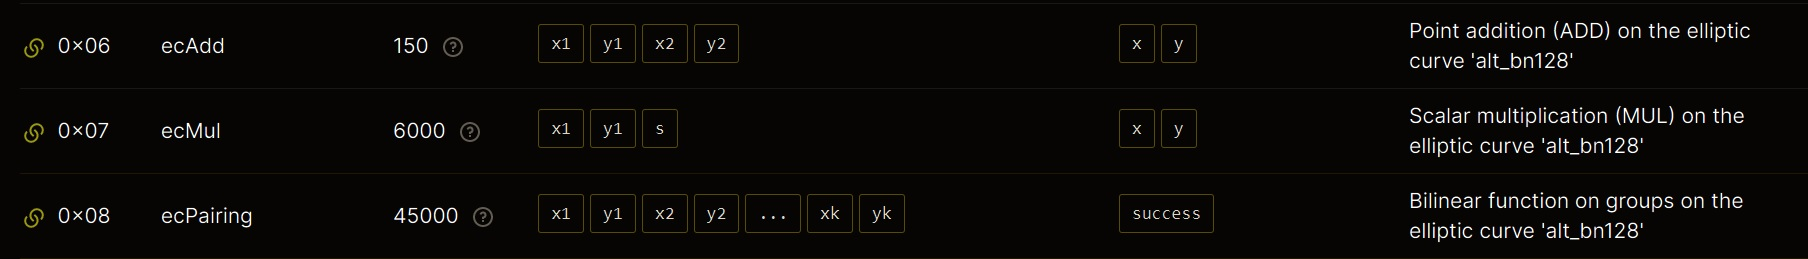
\includegraphics[width=12cm]{images/precompiled.jpg}
 \end{center}
 
Available in Cairo through Nethermind and Garaga.

Notice that the cost of a pairing is x15 compared to a ecRecover (ECDSA).

Not available in Nano. 

\end{frame}


%%%%%%%%%%%%%%%%%%%%%%%%%%%%%%%%
\section{Use cases}

\begin{frame}{Use cases}
\begin{center}
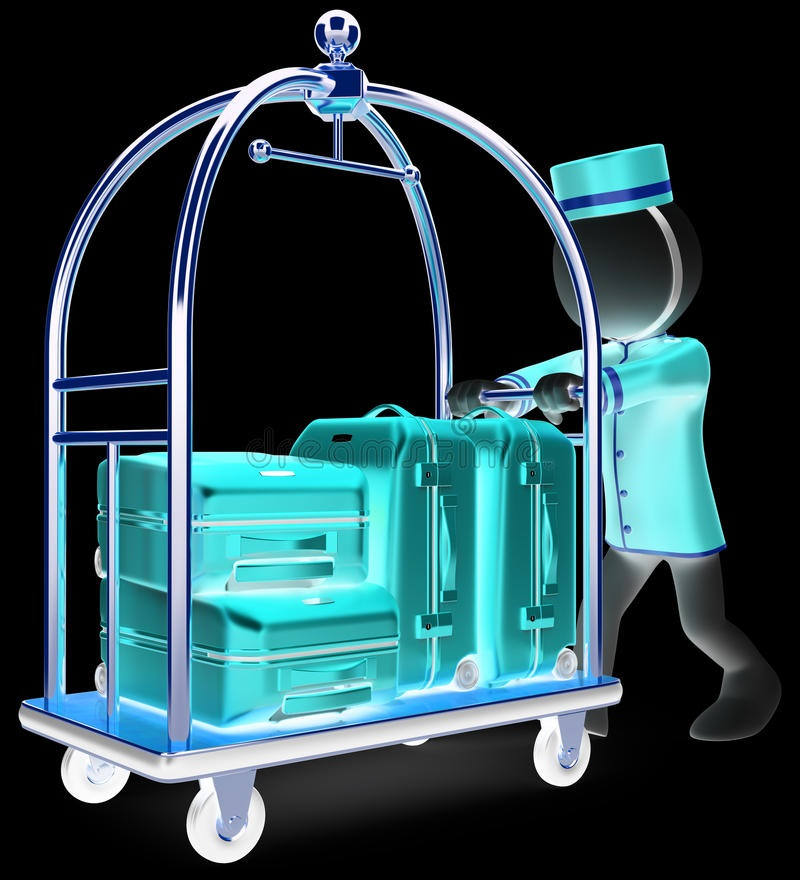
\includegraphics[width=7cm]{images/usecases.jpg}
\end{center}


\end{frame}


%%%%%%%%%%%%%%%%%%%%%%%%%%%%%%%%%%%%%%%%%%%%%%%%
\begin{frame}{ZKProof-of-Ledger :Genuine Check}

\begin{center}
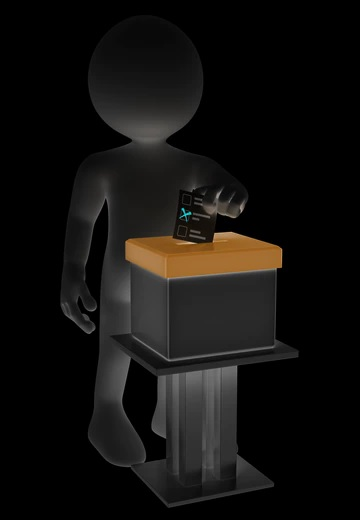
\includegraphics[width=2cm]{images/vote.jpg}
\end{center}

Each time a Nano authenticates, use ECDAA, LL doesn't learn anything other than genuinity.

No linkability required.

The credentials could be deterministically generated for anti replay.

\end{frame}

%%%%%%%%%%%%%%%%%%%%%%%%%%%%%%%%%%%%%%%%%%%%%%%%
\begin{frame}{Safe and Private Infinity Pass: Airdrop}


Each Pass is associated to a set of credentials. Then a drop is linkable (anonymous but only once).


\end{frame}

%%%%%%%%%%%%%%%%%%%%%%%%%%%%%%%%%%%%%%%%%%%%%%%%
\begin{frame}{Voting system}

\begin{center}
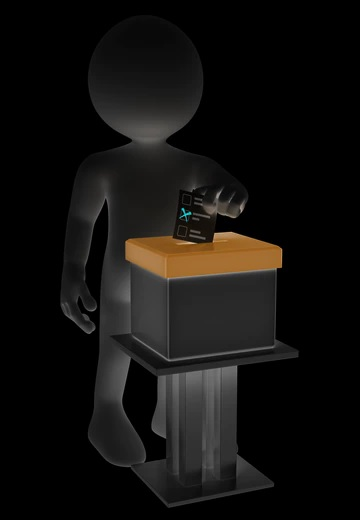
\includegraphics[width=2cm]{images/vote.jpg}
\end{center}

Each vote is a linkable signature of a given message.

Tag='election', Message='Nico President', ECDAA(credentials, Tag, Message).

\end{frame}
%%%%%%%%%%%%%%%%%%%%%%%%%%%%%%%%%%%%%%%%%%%%%%%%

%%%%%%%%%%%%%%%%%%%%%%%%%%%%%%%%%%%%%%%%%%%%%%%%
\section{Ledger Use cases}
\subsection{Ledger and ECDAA}
\begin{frame}


\begin{itemize}
\item Fresh Genuine Check (deployer): (wallet, current development over Argent) over verifier (Cairo) or signer (C)
\item Nano Signer (rust)
\item Device ID
\item Write an EIP/RFC like doc 
\item Some EVM (Polygon) chain for a secure privacy-preserving NFT Pass
\end{itemize} 


Adapt ECDAA to blockchain constraint (curves, hashing).

\end{frame}
%%%%%%%%%%%%%%%%
\section{Starknet and Ethereum ECDAA}
\subsection{Specificities}

\begin{frame}
ECDAA is currently specified by TPM2.0 and 
{\cyan \href{https://fidoalliance.org/specs/fido-v2.0-id-20180227/fido-ecdaa-algorithm-v2.0-id-20180227.html}{Fido2}}
(draft) over specific BN curves.

\only<1>{
Instanciation:
\begin{itemize}
\item use the ASM/TPM architecture with Nano=ASM (authenticator), Phone/Desktop = host
\item issuer : backend
\item verifier : backend for genuine Check, Smarcontract in solidity/cairo for airdrops/fresh endorsement.
\end{itemize}
}

\only<2>{
Necessary modifications:
\begin{itemize}
\item use a pairing friendly curve compatible with EVM,Cairo and Nano : BLS12 and BN254 (PoC on EVM)
\item use the ASM/TPM architecture with Nano=ASM (authenticator), Phone/Desktop = host
\item hash to curve: introduce co-factor clearing to make specification consistent (hash to curve incompatible with BLS)

\end{itemize}

}


\end{frame}

%%%%%%%%%%%%%%%%%%%%%%%%%%%%%%%%%%%%%%%%%%%%%%%%
\subsection{Status}

\begin{frame}{Status}
Current status:

\begin{tabular}{|c|c|c|}
\hline
Target & Completion & Comment \\
\hline
 {\cyan \href{https://github.com/rdubois-crypto/MyCairoPlayground/blob/main/Sage/ECDAA/ecdaa.py}{Simulation}} & 95\% & Add more testing \\ 
 (HLS) && \\
\hline 
 Cairo & 5\% &  working on synchronization of hash over curve \\
\hline 

 Solidity & 10\% & All building blocks synchronized \\
 && Perfect Guild Training ! \\
 \hline 
 Nano & 0\% & Need Dev NanoX\\
 && Grom, let's rust it ! \\
\hline 
 Back end & 0\% & use of HLS for PoC \\
\hline 

\end{tabular}


\end{frame}


%%%%%%%%%%%%%%%%%%%%%%%%%%%%%%%%%%%%%%%%%%%%%%%%

%%%%%%%%%%%%%%%%%%%%%%%%%%%%%%%%%%%%%%%%%%%%%%%%
    \section{}
    \begin{frame}{}
        \centering
            {\Huge\bfseries
        \textcolor{yellow}{Questions ?}}
        
            
\includegraphics[width=8cm]{images/questions.jpg}
            
           \begin{tabular}{ccc}
           \href{https://github.com/rdubois-crypto/CYLIB-Speculos}{\cyan{C Library}} & ~~~~~~~~~~~~~~~~~~\href{https://github.com/rdubois-crypto/MyCairoPlayground/tree/main/slides}{\cyan{Slides }} ~~~~~~~~~~~~~~~~~~&   \href{https://github.com/rdubois-crypto/MyCairoPlayground}{\cyan{Cairo\&Sage }}\\
            
           
\includegraphics[width=2cm]{images/musig2_qr.jpg} & 
\includegraphics[width=2.1cm]{images/qrslides.jpg} &
\includegraphics[width=2.1cm]{images/cairomusig2_qr.jpg}
            \\
           \end{tabular}     		
    \end{frame}
\end{document}

  
% https://en.wikipedia.org/wiki/Privacy
% [CL16]: Concepts Around Privacy-Preserving Attribute-Based CredentialsJan Camenisch  https://hal.archives-ouvertes.fr/hal-01276046/document
